\documentclass[11pt,a4paper,titlepage]{article}

\usepackage{pdflscape}
\usepackage[margin=1in]{geometry}
\usepackage{titling}
\usepackage{graphicx}
\usepackage{titlesec}
\usepackage[hidelinks]{hyperref} 

\graphicspath{ {./Images/} }

\setcounter{secnumdepth}{4}

\titleformat{\paragraph}
{\normalfont\normalsize\bfseries}{\theparagraph}{1em}{}
\titlespacing*{\paragraph}
{0pt}{3.25ex plus 1ex minus .2ex}{1.5ex plus .2ex}

\begin{document}
%\title{ \huge Functional Requirements for the SAMBUG}

\begin{titlepage}
	
	
	\begin{center}
		\vspace*{-3cm}
  		\makebox[\textwidth]{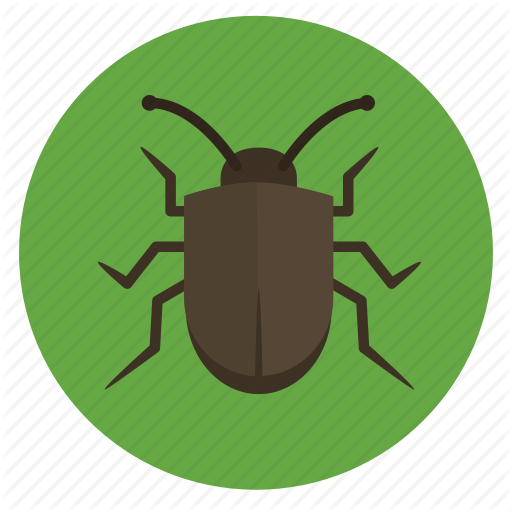
\includegraphics[width=\paperwidth]{sambug}}
	\end{center}
	
	%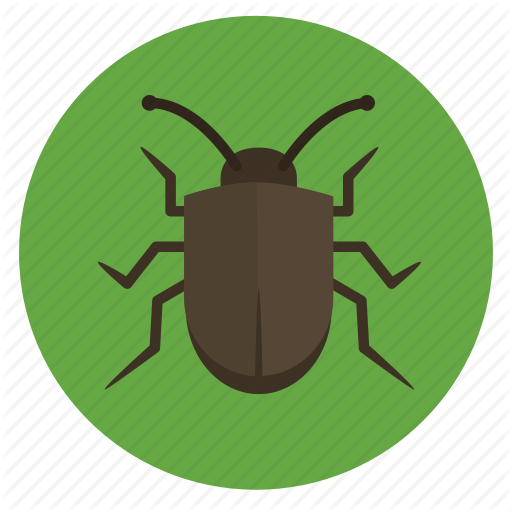
\includegraphics[width=\paperwidth]{sambug}
	
    \vspace*{2cm}
      \Huge \textbf {SAMBUG}\\
      
    \vspace*{-0.5cm}
	  \huge \textbf {User Manual}\\
	  
	\vspace*{-0.5cm}  
      \LARGE \textbf {Subtrop}
         
    \vskip2cm
          
    
    \large \textbf{July, 2015}
    \vfill
\end{titlepage}
	
	

\tableofcontents

\pagebreak

\section{System Overview}
The main goal of the SAMBUG system is to help Macadamia nut farmers (or any other farmers dealing with stink bugs as a pest). Please note that this system was developed with specific work flows in mind, which will be addressed later. 
The farmers can use the system in two ways, namely an Android application and a browser interface.\\\\
The way in which the system will help farmers will be listed below:
	\begin{itemize}
		\item Farmers can easily use the Android application to classify 			stink bugs while in the field. These bugs may be part of a sample 		that was taken during scouting. Classification can be done using 			two methods, manual classification and automatic classification:
		\begin{itemize}
			\item \textbf{Manual Classification:} This method allows the 				user to take a photo of a specific bug (one at a time) and 					then selecting another photo from a gallery. This photo must 				be chosen to most resemble the bug of which the initial photo 			was taken. The application makes this easy by placing the 					captured image next to the possible selected photo to make 					comparison easier.
			\item \textbf{Automatic Classification:} This method also 					allows the user to take a photo of the specific bug, and 					thereafter the application will do the classification. This 				classification is done using artificial intelligent systems. 				Automatic classification will be more accurate than manual 					classification. 
		\end{itemize}
		\item While scouting and classifying bugs, the application makes 
		it easy to enter additional data, such as the number of that 				specific bug that was found, in which block of the far it was. 				etc.
		\item After doing a scout trip, a summary will be shown, 					summarising the number and types of bugs found during that trip. 			Using this summary, farmers can decide with more confidence if 				spraying pesticide is necessary or not.
		\item When taking a photo during classification, the geolocation 			will be taken as well. With this feature, farmers will find it 				easier to make sure that scouts actually go out to random 					locations.
		\item After capturing the data for a scout trip, this data will 			be stored in a database such as to later look back at the data.
		\item The browser interface can be used by the farmers to manage 			his/her farm and to view data from previous scout trips. It will 			be able to view the data through means of graphs and also tables. 		Various filters can then be applied to these graphs and tables, 			such as blocks and dates, making it easier to draw conclusions.
	\end{itemize}
\section{System Configuration}

\section{Installation}
		
\section{Getting started}

\section{Using the system}

\section{Troubleshooting}

\end{document}

%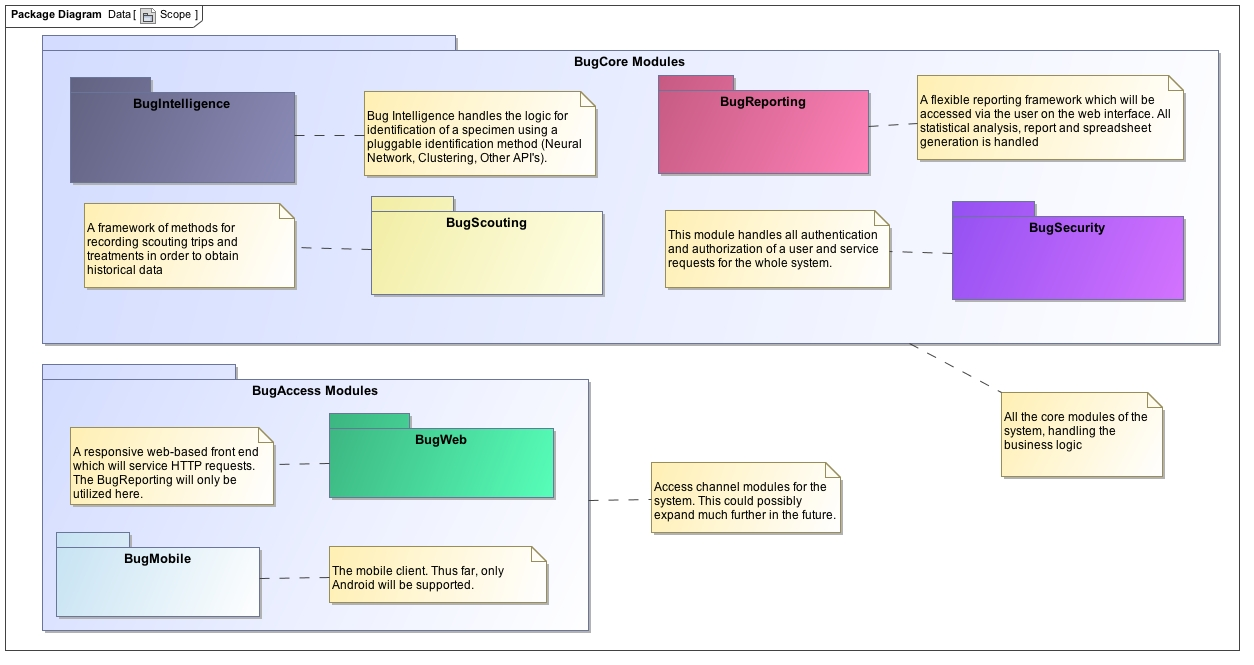
\includegraphics[width=\linewidth]{scope}